
\subsubsection{KW45: 08.11.2021 bis 14.11.2021}
\begin{quote}
	\subsubsection*{Arbeit in der Schule}
	Da der Gargoyle Charakter nicht funktioniert hat habe ich die Schritte nochmals wiederholt.
	- import vom JL-Game folgendes: JohnLemon, Gargoyle, FaderCanvas
	
	- export in das eigene Spiel
	
	- Prefab Modelle von JohnLemon und Gargoyle in die Scene eingefügt
	
	- FaderCanvas prefab eingefügt welches folgende Bilder beinhaltet:
		-ExitlmageBackground
		-CaughtlmageBackground
		
	  Der CaughtImage wird angezeigt wenn der Gargoyle Charakter den Haupcharakter in seiner PointOfView hat.
	  
	- Das PrefabModell GameEnding wurde auch vom JL-Game importiert.
	  Funktion von GameEnding: wenn der Character den Ziel(GameEnding Cube) erreicht, wird ExitlmageBackground angezeigt.
	  
	- Ergebnis: Wenn J.L im Blickwinkel vom Gargoyle ist wird Caughtlmage angezeigt und wenn J.L das Ziel erreicht wird Exitlmage angezeigt.
	
	- Das GameEnding Programm wurde im J.L Kurs in den Sommerferien geschrieben.
	
	 Abbildung \ref{fig:gameviewsskw45131122}
	  \begin{figure}
	  	\centering
	  	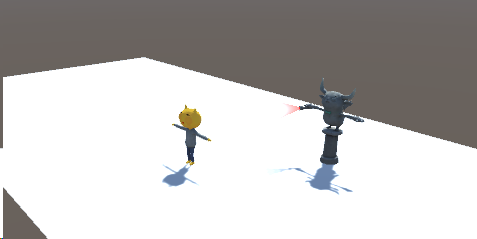
\includegraphics[width=0.5\linewidth]{img/SemihSoenmez_IMG/GameView_SS_KW45_131122}
	  	\caption{}
	  	\label{fig:gameviewsskw45131122}
	  \end{figure}
	\subsubsection*{Arbeit außerhalb der Schule}
	-Das Programm soll jetzt auch für unsere Charaktere funktionieren.
	
	 Unsere Charaktere: Hauptcharakter Schüler: Abbildung\ref{fig:main-charaktersskw45131121}
	 
	 Lehrer Charakter: Abbildung \ref{fig:lehrercharakterss151121}
	 \begin{figure}
	 \centering
	 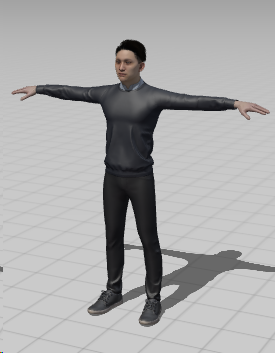
\includegraphics[width=0.3\linewidth]{img/SemihSoenmez_IMG/LehrerCharakter_SS_151121}
	 \caption{}
	 \label{fig:lehrercharakterss151121}
	 \end{figure}
	 					
	 					
	- Hauptcharakter Schüler wurde in die Scene eingefügt und die Parameter von Gargoyle für den Hauptcharakter angepasst.
	
	Ergebnis: Gargoyle erkennt den Hauptcharakter.
	
	- Charakter Lehrer wurde in die Scene eingefügt.
	
	
	
	\subsubsection*{Was ist geplant für die Nächste Woche}
	Die Funktion vom Charakter Gargoyle soll dem Charakter Lehrer implementiert werden.
	Ein dynamischer Gegner soll entwickelt werden, wie z.B. der Charakter Ghost.
	
	\subsubsection*{Welche Schwierigkeiten hat es gegeben}
	Die Funktionen von Charakteren richtig Laufen zu bringen.
	
\end{quote}
